\chapter{Methodology}\label{ch:3}
This chapter delineates the comprehensive and systematic methodology employed to develop and evaluate a sophisticated classification pipeline capable of determining course equivalency from domain-specific textual data. As established in the preceding chapters, the manual nature of course articulation creates significant barriers for students. Furthermore, as discussed in Chapter~\ref{ch:2}, previous automated approaches have faced significant limitations related to data privacy, scalability, and interpretability, indicating a need for a new paradigm~\cite{pardos-articulation-2019, slade10.1177/0002764213479366}.

To address these challenges, the research followed an evolutionary, two-phase process. The investigation commenced with an initial, exploratory phase to assess the feasibility of using Large Language Models (LLMs) as end-to-end classifiers. The findings from this stage were informative; they demonstrated the potential of modern LLMs but also highlighted significant limitations that motivated the development of a more robust and scalable framework. Consequently, the primary focus of this thesis is a more advanced, decoupled methodology that utilizes deep embedding models as sophisticated feature extraction engines.

This chapter details this entire methodological journey. It begins by describing the initial direct LLM classification approach and the findings that motivated the subsequent pivot. It then details the final pipeline's core components: the data corpora, the feature engineering process, the selection and fine-tuning of deep embedding models, and the suite of downstream classifiers. Finally, by outlining the complete evaluation framework, including performance metrics, statistical analyses, and error analysis methodologies, this chapter sets a clear and rigorous stage for the discussion of results in Chapter~\ref{ch:4}.

\section{Phase 1: Direct LLM Classification Approach}\label{ch:3.1}
The research commenced with an exploratory phase designed to determine the feasibility of leveraging Large Language Models (LLMs) as end-to-end classifiers for the course equivalency task. This direct approach was a pragmatic first step, conceived as an initial benchmark to establish a baseline for performance using a small, manually curated dataset. At this stage of the research, a larger, more comprehensive dataset from the Program Pathways Mapper (PPM) was anticipated but not yet available, making a focused, smaller-scale investigation the most logical starting point. This methodology treated the LLM as a holistic reasoning engine, tasked with performing the entire classification from raw text input to a final equivalency judgment without intermediate feature engineering.

\subsection{Initial Data Corpus and Pre-processing}\label{ch:3.1.1}
The dataset for this initial evaluation was constructed to represent a challenging, real-world scenario using publicly available data. The process began by identifying five required lower-division courses for the Computer Science major at San Francisco State University (SFSU). Using ASSIST, articulation agreements were found for these courses across 63 different California public colleges and universities. The raw course data was then manually collected from the online course catalogs of each respective college. This data consisted of the full, unmodified text including department codes, course numbers, titles, descriptions, and all associated metadata such as prerequisites, unit counts, and grading options. This approach was deliberately chosen to ensure that the analysis could compare the effectiveness of classification using the complete raw text versus more structured, extracted information.

The initial dataset consisted of 228 equivalent course pairs based on the articulation agreements (see Table~\ref{tbl:sfsucourses}). To create a more robust dataset for binary classification, this set was expanded by assuming symmetry and transitivity for course equivalency, which generated a total of 5,660 equivalent pairs. An equivalent number of non-equivalent pairs was then generated by randomly pairing courses from different subjects. From this expanded corpus of over 11,000 pairs, a final stratified random sample of 400 pairs (200 equivalent and 200 non-equivalent) was created to serve as the evaluation set for the models.

\begin{table}[tb]
    \captionsetup{skip=5pt}
    \centering
    \caption{SFSU Courses Identified}
    \begin{tabular}{rlc}
        \toprule
        \textbf{Code$^{\mathrm{a}}$} & \textbf{Title}                & \textbf{Count} \\
        \midrule
        MATH 226                     & Calculus I
                                        & 61                                             \\
        CSC 210                      & Intro to Computer Programming
                                        & 51                                             \\
        CSC 220                      & Data Structures
                                        & 44                                             \\
        CSC 230                      & Discrete Math
                                        & 47                                             \\
        CSC 256                      & Machine Structures
                                        & 25                                             \\
        \bottomrule
        \multicolumn{3}{l}{$^{\mathrm{a}}$Course code from San Francisco
            State University course catalog}
    \end{tabular}
    \label{tbl:sfsucourses}
\end{table}

\subsection{Model Selection and Prompt Engineering}\label{ch:3.1.2}
An preliminary review of various LLMs was conducted to assess their ability to reliably generate structured data from the raw course descriptions. While many open-source and proprietary models were tested, Google's PaLM2 and its successor, Gemini Pro v1.0, were ultimately selected for this phase of the research. This decision was based on their accessibility via a free-tier API and, most importantly, their consistent ability to produce well-formatted, structured data from the unprocessed text.

A structured, iterative prompt engineering process, illustrated by Figure~\ref{fig:prompt_engineering_process}, was employed to develop effective prompts for both the extraction of structured data (like course topics) and the final equivalency classification. This process involved starting with simple prompts and gradually refining them based on established design principles from natural language processing research and community guides~\cite{ye2024promptengineeringpromptengineer,ppp,peg}. The final prompts for data extraction were highly structured, consisting of five parts: a preamble summarizing the task, the raw course data, specific formatting instructions, a JSON model schema defining the desired output, and a postamble with additional clarifying instructions. A complete prompt template examples can be found in Appendix~\ref{app:llmprompts}. Despite this careful refinement, the structured data extraction process, particularly for deducing course topics, remained a significant challenge and was prone to occasional contextual errors.

\begin{figure}[tb]
    \captionsetup{skip=5pt}
    \centering
    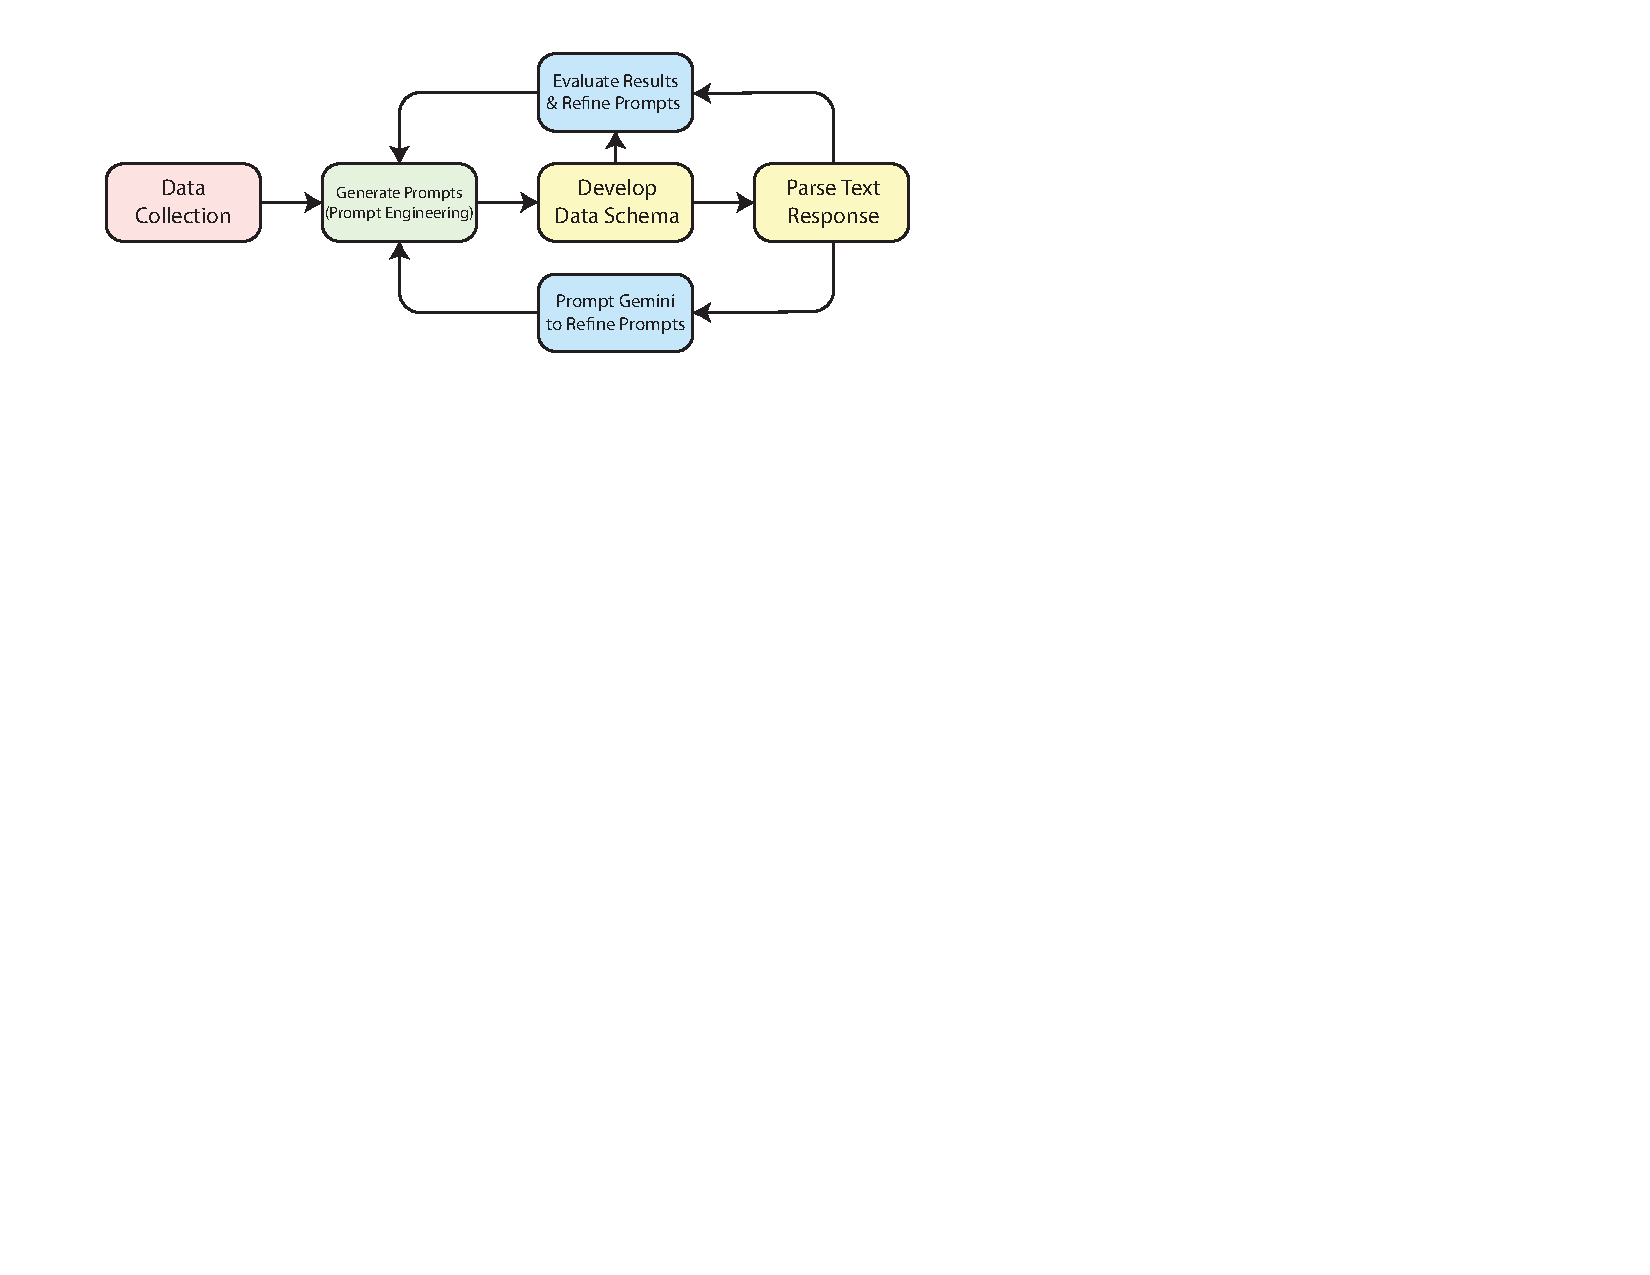
\includegraphics[scale=1,trim={0 0 0 0},clip]{prompt_engineering_flow.pdf}
    \caption{Prompt Engineering Process}
    \label{fig:prompt_engineering_process}
\end{figure}

\section{Phase 2: The Decoupled Pipeline Framework}\label{ch:3.2}
The limitations identified in the initial study—including high computational cost, lack of quantifiable similarity scores, and prompt sensitivity—directly motivated a pivot to a more sophisticated, decoupled pipeline. This new approach was first developed and prototyped using the initial, manually-curated dataset. This section details this final, more robust methodology, beginning with the larger and more comprehensive data corpus upon which it was ultimately trained and validated.  The complete pipeline workflow is illustrated in Figure~\ref{fig:ftpipeline}.

\begin{figure}[tb]
    \captionsetup{skip=5pt}
    \centering
    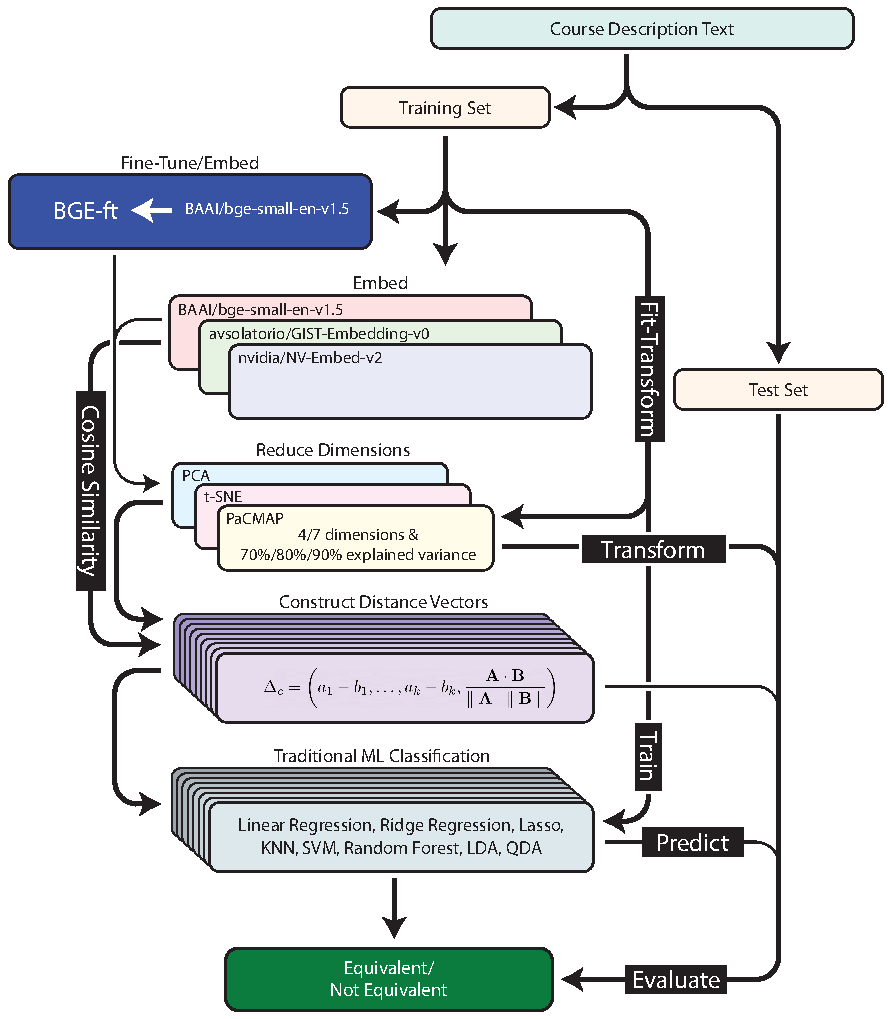
\includegraphics[width=0.75\linewidth,trim={0 0 0 0},clip]{methodsworkflow.pdf}
    \caption{The Decoupled Pipeline Framework}
    \label{fig:ftpipeline}
\end{figure}

\subsection{The PPM Corpus and Data Preparation}\label{ch:3.2.1}
The limitations of the initial study necessitated not only a more sophisticated methodology but also a larger, more comprehensive dataset to robustly train and evaluate it. This required data corpus was procured at a later stage of the research in partnership with the Program Pathways Mapper (PPM). The acquisition of this dataset was a critical step that enabled the full-scale implementation and validation of the decoupled pipeline.

The corpus provided by the PPM initially contained 2,217 courses, each labeled with a Course Identification Numbering System (C-ID) code that serves as the ground truth for course equivalency. To prepare this data for a robust, stratified partitioning, a critical filtering step was applied first. All C-ID classes with fewer than four associated courses were removed from the dataset. This step was essential to guarantee that after splitting the data, both the training and subsequent test sets would contain enough examples to form at least one equivalent course pair for every class, a necessary condition for the fine-tuning process. This filtering resulted in a final, clean corpus of 2,157 courses distributed across 157 distinct C-ID classes.

To ensure a rigorous and unbiased evaluation of the final models, this final dataset was partitioned into two distinct, non-overlapping subsets: a training set and a test set. A stratified 50/50 split was employed, using the C-ID code as the stratification key. This resulted in a training set of 1,078 courses and a test set of 1,079 courses. The stratification ensures that each of the 157 classes is represented in both subsets. From the training and test sets, a total of 8672 and 9192 course pairs were generated, which had a 50/50 split of equivalent and non-equivalent course pairs (see Table~\ref{tbl:ppmdatasplit}).  The test set is held in reserve and used only once for the final, conclusive evaluation of the optimized classification pipeline, providing an honest estimate of the model's generalization performance on unseen data.

\begin{table}[tb]
    \captionsetup{skip=5pt}
    \centering
    \caption{PPM Data Split}
    \begin{tabular}{lccc}
        \toprule
        \textbf{Data Set} & \textbf{Equivalent} & \textbf{Non-Equivalent} & \textbf{Total} \\
        \midrule
        Training     & 4336  & 4336    &  8672                                       \\
        Test         & 4596  & 4596    &  9192                                   \\
        \bottomrule
    \end{tabular}
    \label{tbl:ppmdatasplit}
\end{table}

\subsection{Input Document Normalization}\label{ch:3.2.2}
In a departure from conventional NLP pipelines, this research deliberately eschewed standard text pre-processing techniques such as lowercasing, stop-word removal, or the stripping of special characters. This decision was made to more accurately simulate a real-world use case where input data may be imperfectly formatted. The methodology, therefore, relies on the inherent semantic power and robustness of modern transformer-based embedding models to interpret and handle this ``raw'' text.

Instead of cleaning the text, a normalization step was performed to create a consistent, structured input document for the embedding models. A new field, ``Formatted Course Info,'' illustrated in Table~\ref{tbl:formattedcourse}, was generated for each course by concatenating four key pieces of information: the department name, the department course number, the course title, and the full course description. This concatenated string serves as the single document representation for each course and is the direct input for the document embedding process, ensuring all relevant textual context is preserved in a standardized format.

\begin{table}[tb]
    \captionsetup{skip=5pt}
    \centering
    \caption{Example of Formatted Course Info}
    \begin{tabular}{p{0.45\textwidth}p{0.5\textwidth}}
        \toprule
        \textbf{Template} & \textbf{Example} \\
        \midrule
        \small
        \(\langle\)Dept Code\(\rangle\)-\(\langle\)Course Code\(\rangle\) \(\langle\)Course Title\(\rangle\)     & 
    \small CSC-215  Intermediate Computer Programming \\
        
    \small \(\langle\)Course Description\(\rangle\) &  
    \small Prerequisite: CSC 101 with a grade of C or better. \\
        & 
    \small Design, implementation, testing, debugging, maintenance, and documentation of Java programs. Algorithms, programming concepts, and data types in Java. Concepts of object-oriented programming. Numerical and non-numerical problems. Hands-on exercises in programming, and the use of basic software development tools. \\
        \bottomrule
    \end{tabular}
    \label{tbl:formattedcourse}
\end{table}

\subsection{Feature Engineering}\label{ch:3.2.3}
The high-dimensional embedding vectors generated by the models, while semantically rich, are not the final features used for classification. To prepare the data for the downstream classifiers, a two-stage feature engineering pipeline was executed. This pipeline first applies various dimensionality reduction techniques and then constructs pairwise difference vectors from these embeddings to explicitly represent the relationship between two courses.

\subsubsection{Dimensionality Reduction}\label{ch:3.2.3.1}
The high-dimensional vectors produced by modern embedding models can present challenges for downstream machine learning algorithms, a phenomenon often referred to as the ``curse of dimensionality.'' To address these potential issues, a methodical process of dimensionality reduction was applied. This investigation was motivated by several potential benefits, including improving model generalization by removing redundant or noisy dimensions and reducing computational complexity.

To ensure the integrity of the evaluation and prevent any form of data leakage, the reduction models were governed by a strict protocol. Each reduction technique was fit exclusively on the training data. The same fitted model was then used to transform both the training and the held-out test sets. This methodology guarantees that no information from the test set influences the parameters of the reduction models. A comprehensive exploration was conducted to determine the optimal dimensionality, including using Principal Component Analysis (PCA) to reduce vectors to the number of components required to explain 70\%, 80\%, and 90\% of the original variance, as well as reducing to static 4 and 7 dimensions using PCA, t-SNE, and PaCMAP.

\subsubsection{Composite Distance Vector}\label{ch:3.2.3.2}
The ultimate goal of this research is to classify pairs of courses, which requires input features that represent the relationship between them. To provide a richer, more discriminative representation than a single metric alone, we designed a composite feature vector, \(\Delta_c\). The vector is constructed by concatenating the element-wise difference of the two course embedding vectors (\(\mathbf{A}\) and \(\mathbf{B}\)) with their cosine similarity:
\[ \Delta_c = \left(a_1 - b_1, \dots, a_k - b_k, \frac{\mathbf{A}\cdot\mathbf{B}}{\parallel \mathbf{A} \parallel \parallel \mathbf{B} \parallel } \right) \]
where \(\mathbf{A} = (a_1, \dots, a_k) \) and \(\mathbf{B} = (b_1, \dots, b_k) \) are the \(k\)-dimensional embedding vectors for the two courses. This design is powerful because it provides the subsequent classifier with two distinct types of information simultaneously. The element-wise difference captures granular, dimension-specific (local) disparities between the two semantic representations, while the cosine similarity provides a single, normalized measure of their overall (global) alignment in the vector space. A custom \verb|CoursePairGenerator| class, found in the project's codebase, was implemented to generate these feature vectors for all positive and negative pairs across all embedding and reduction variations.

\section{Model Architecture and Training}\label{ch:3.3}
A central hypothesis of this research is that a generic, pre-trained deep embedding model can be adapted to produce highly specialized and semantically rich embeddings for the specific domain of course descriptions. These bespoke embeddings are expected to provide a more discriminative feature representation for downstream classification tasks compared to off-the-shelf models. This section details the architecture, learning objective, and training protocol used to achieve this adaptation through a process of deep metric learning, as well as the downstream classifiers used to evaluate the resulting features.

\subsection{Embedding Models: Selection and Fine-Tuning}\label{ch:3.3.1}
The selection of an appropriate embedding model is a critical first step that influences the entire downstream pipeline. Rather than committing to a single model, this research began with a broad preliminary analysis of a variety of open-source embedding models to identify strong candidates for a more in-depth, comparative study.

\subsubsection{Model Selection}\label{ch:3.3.1.1}
The initial models reviewed, summarized in Table~\ref{tbl:emb_models}, spanned a wide range of parameter sizes and characteristics. To screen these models efficiently, the simple but effective cosine similarity accuracy metric was used: for a given anchor course, a model was considered correct if the cosine similarity to an equivalent course was greater than the similarity to a non-equivalent course. This initial screening revealed that while performance varied, many models achieved high accuracy. Based on these results and a desire to evaluate a representative spectrum of model sizes, three models were selected for the primary analysis:
\begin{itemize}
    \item \verb|BAAI/bge-small-en-v1.5| (BGE): Representing a high-performing small model.
    \item \verb|avsolatorio/GIST-Embedding-v0| (GIST): Representing a medium-sized model.
    \item \verb|nvidia/NV-Embed-v2| (NVE): Representing a large-scale model.
\end{itemize}
At a later stage of the research, \verb|Salesforce/SFR-Embedding-2_R| (SFR) was also included for additional comparison due to its strong performance on public leaderboards. The foundational architecture for all these models is the transformer, which allows them to generate rich, contextual embeddings suitable for feature extraction.
\begin{table}[!tb]
    \captionsetup{skip=5pt}
    \centering
    \caption{Initial Embedding Model Review}
    \label{tbl:emb_models}
    \begin{tabular}{lcccc}
        \toprule
        Model Name                 & Rank$^{*}$ & Params$^{\dagger}$ & Dims & Acc             \\
        \midrule
        GIST-small-Embedding-v0    & 41         & 33                 & 384  & 0.9759          \\
        bge-small-en-v1.5          & 47         & 33                 & 384  & 0.9670          \\
        GIST-Embedding-v0          & 33         & 109                & 768  & 0.9768          \\
        bge-base-en-v1.5           & 35         & 109                & 768  & 0.9732          \\
        gte-base-en-v1.5           & 31         & 137                & 768  & 0.9732          \\
        mxbai-embed-large-v1       & 24         & 335                & 1024 & 0.9759          \\
        gte-large-en-v1.5          & 21         & 434                & 1024 & 0.9777          \\
        multilingual-e5-large-inst & 34         & 560                & 514  & 0.9670          \\
        stella\_en\_1.5B\_v5       & 3          & 1543               & 8192 & 0.9857          \\
        SFR-Embedding-2\_R         & 4          & 7111               & 4096 & \textbf{0.9839} \\
        Agte-Qwen2-7B-instruct     & 5          & 7613               & 3584 & 0.9804          \\
        nvidia/NV-Embed-v2         & 1          & 7851               & 4096 & 0.9831          \\
        \bottomrule
        \multicolumn{4}{p{6cm}}{\scriptsize $^{*}$ Huggingface Overall Leaderboard Rank} \\
        \multicolumn{4}{p{6cm}}{\scriptsize $^{\dagger}$ in Millions}
    \end{tabular}
\end{table}

\subsubsection{Metric Learning with Batch Triplet Loss Functions}\label{ch:3.3.1.2}
To determine if performance could be further improved, the BGE model was subjected to a fine-tuning process using a deep metric learning approach. Metric learning aims to learn a direct mapping from a high-dimensional input to a compact Euclidean embedding space where the geometric distance between vectors directly corresponds to a measure of semantic similarity. This technique was famously and effectively employed by the FaceNet system~\cite{Schroff_2015}, which used a Triplet Loss function to learn a unified embedding for face recognition. This thesis adapts this proven approach, translating it from the domain of computer vision to the domain of semantic text similarity.

The concept of Triplet Loss, first introduced in the context of face recognition, has been widely applied to supervised similarity learning~\cite{Yu2020}. It operates on (Anchor, Positive, Negative) triplets. The fundamental goal is to train the embedding function, \(f(x)\), to map inputs into a vector space where the distance between an anchor sample (\(A\)) and a positive sample (\(P\)) is smaller than the distance to a negative sample (\(N\)) from a different class, enforced by a margin, \(\alpha\). The mathematical formulation is given by:
\[ L(A,P,N)=\max(d(f(A),f(P))-d(f(A),f(N))+\alpha,0). \]
Here, \(d\) represents the Euclidean distance. The \(\max()\) component ensures that loss is only incurred for triplets that violate the margin constraint. A naive ``offline'' implementation of Triplet Loss that forms all possible triplets is computationally infeasible. A more effective approach is ``online'' mining, where informative triplets are selected on-the-fly from within each mini-batch. This empirical evaluation is motivated by research demonstrating that selecting the ``hardest'' positive and negative examples within each mini-batch is a highly effective strategy for training deep metric learning models~\cite{hermans2017defensetripletlossperson}.  Recognizing that different triplet mining strategies can significantly impact model performance, we empirically evaluated all four primary batch-based triplet loss implementations available in the \verb|sentence-transformers| library:
\begin{itemize}
    \item \textbf{BatchAllTripletLoss}: Computes the loss for all valid triplets within a batch. While comprehensive, the learning signal can be diluted by the high number of ``easy'' triplets.
    \item \textbf{BatchSemiHardTripletLoss}: Considers only semi-hard triplets, where the negative sample is more distant than the positive but still violates the margin. This is a common strategy that balances stability and learning effectiveness.
    \item \textbf{BatchHardTripletLoss}: Implements a more aggressive strategy, using the hardest positive and hardest negative for each anchor. This can accelerate convergence but can also be ``temperamental'' and lead to a noisy optimization landscape.
    \item \textbf{BatchHardSoftMarginTripletLoss}: A variation of \verb|BatchHardTripletLoss| that does not require a manually specified margin parameter, simplifying hyperparameter tuning.
\end{itemize}

\subsubsection{Optimization and Training Protocol}\label{ch:3.3.1.3}
The successful fine-tuning of a model with a challenging objective like \verb|BatchHardTripletLoss| is critically dependent on the choice of optimizer and learning rate schedule. The components selected for this research were not chosen in isolation but as parts of a cohesive, synergistic framework designed to ensure stable and effective learning.{\setlength{\emergencystretch}{5em}\par}

The optimization of the model's weights was performed using the AdamW optimizer. Proposed by Loshchilov and Hutter, AdamW improves upon the standard Adam optimizer by addressing a subtle flaw in how it handles L2 regularization~\cite{loshchilov2019decoupledweightdecayregularization}. In the standard Adam optimizer, weight decay is coupled with the adaptive gradient calculation, which can lead to suboptimal regularization and poorer generalization. AdamW decouples the weight decay from the gradient update, applying it directly to the weights as originally intended. This results in more stable training and improved model generalization, which is particularly crucial when dealing with the noisy gradients that can arise from hard-negative mining strategies.  This ensures a more stable and effective regularization, which is crucial for preventing the model from overfitting, particularly given the noisy gradients that can arise from hard-negative mining~\cite{loshchilov2019decoupledweightdecayregularization}.

The optimizer was paired with the \verb|CosineAnnealingWarmRestarts| learning rate schedule. This scheduler, also introduced by Loshchilov and Hutter~\cite{loshchilovhutter}, was chosen to address the challenge of navigating the complex, non-convex loss landscapes that can arise from triplet loss, where an optimizer can become trapped in sharp, suboptimal local minima.  Two powerful concepts drive this schedule: cosine annealing, which smoothly decays the learning rate following a cosine curve, and ``warm restarts,'' where the rate is periodically reset to its initial maximum~\cite{pytorchcosanneal}. By allowing the optimizer to escape suboptimal local minima that it may have settled into and explore other regions of the complex loss landscape, the scheduler increases the likelihood of finding a higher-quality solution~\cite{loshchilovhutter}.

Finally, the data loading and batching strategy was intrinsically linked to the fine-tuning objective. A crucial constraint of the triplet loss functions is that the training data must contain a minimum of two examples for each class label to form a valid (anchor, positive) pair~\cite{sbertLosses}. To mitigate the risk of creating mini-batches that fail this constraint through simple random sampling, this research leveraged the \verb|GroupByLabelBatchSampler| from the \verb|sentence-transformers| library. This sampler ensures that each mini-batch is constructed by grouping samples with the same label, thereby guaranteeing every batch contains the necessary class diversity to form valid and informative triplets for all anchors~\cite{sbertSamplers}.

\subsection{Downstream Classification Models}\label{ch:3.3.2}
To determine the most effective method for classifying the generated pairwise feature vectors, a broad suite of machine learning algorithms was evaluated. The process began with a comprehensive initial evaluation of eight different models to understand which algorithmic families were best suited to the data. This initial suite included:
\begin{itemize}
    \item \textbf{Linear Models (Logistic Regression, Ridge, Lasso)}: To establish a baseline and test for linear separability.
    \item \textbf{Instance-Based Model (k-Nearest Neighbors)}: To probe the local structure and clustering of the feature space.
    \item \textbf{Kernel-Based Model (Support Vector Machine)}: To test for complex, non-linear decision boundaries.
    \item \textbf{Ensemble Model (Random Forest)}: For its robustness and ability to capture complex feature interactions.
    \item \textbf{Probabilistic Models (LDA and QDA)}: To test assumptions about the geometric distribution of the data.
\end{itemize}
Based on the preliminary results from this comprehensive evaluation, four models were selected for the final, in-depth analysis due to their consistently strong performance: K-Nearest Neighbors (KNN), Support Vector Machine (SVM), Random Forest (RF), and XGBoost. XGBoost, a powerful gradient boosting implementation, was added at this stage to include a state-of-the-art boosting algorithm known for its high performance on structured data, ensuring the final comparison was robust and comprehensive.

\section{Evaluation Framework and Metrics}\label{ch:3.4}
A rigorous, multi-stage evaluation framework was designed to narrow down the optimal combination of embedding models, dimensionality reduction techniques, and classifiers, and to provide a comprehensive view of the entire pipeline's performance. This section details the design of that framework, the metrics used to measure performance, and the statistical methods planned for the final analysis.

\subsection{Multi-Stage Evaluation Design}\label{ch:3.4.1}
The evaluation process was designed as a funnel, beginning with a broad preliminary review to efficiently narrow the field of candidates, followed by a more focused and rigorous analysis on the larger, more comprehensive PPM Corpus.

\subsubsection{Stage 1: Initial LLM Feasibility and Benchmark}
The process began with a broad analysis to assess the feasibility of using a Large Language Model for direct classification and to contextualize its performance. This stage, conducted on the Initial Dataset, involved two parts:
\begin{enumerate}
    \item \textbf{Feasibility Study}: The primary evaluation tested Google's Gemini Pro v1.0 across different input data types (full raw text vs. extracted topics) and three classification schemes (binary, 3-way, and 4-way) to understand its capabilities and limitations.
    \item \textbf{Comparative Benchmark}: To contextualize the results, a comparative analysis was conducted against a suite of other prominent open-source LLMs using the same binary classification task.
\end{enumerate}

\subsubsection{Stage 2: Feature Vector Validation (Ablation Study)}\label{ch:3.4.1.1}
A critical ablation study was designed to validate the efficacy of the novel composite distance vector, \(\Delta_c\). This involved training the full suite of initial classifiers on two different versions of the feature set derived from the Initial Dataset: one using the complete composite vector and one using an ablated vector containing only the element-wise differences. By comparing the performance across these two conditions, it was possible to isolate and measure the contribution of the global cosine similarity feature.

\subsubsection{Stage 3: Evaluation During Fine-Tuning}\label{ch:3.4.1.2}
With the larger, more robust PPM dataset, the most promising non-proprietary embedding models were fine-tuned to specialize them for the course equivalency task. To monitor the quality of the learned embeddings during this process, the \verb|BinaryClassificationEvaluator| from the \verb|sentence-transformers| library was employed. At the end of each training epoch, the evaluator was run on binary-labeled course pairs generated from the training set. The primary metric monitored was Average Precision based on cosine similarity, and the model checkpoint that achieved the highest score on these validation pairs was saved as the best model for that fine-tuning run.{\setlength{\emergencystretch}{5em}\par}

\subsubsection{Stage 4: Final Downstream Classifier Evaluation}\label{ch:3.4.1.3}
The final and definitive evaluation was conducted on the held-out test portion of the PPM dataset. This stage used the feature vectors generated from the best-performing embedding models (both the original off-the-shelf versions and the newly fine-tuned versions). These feature sets were then used to train and evaluate the final selection of high-performing classifiers: KNN, Random Forest, SVM, and XGBoost. This ensures an unbiased assessment of the complete pipeline's ability to generalize to new, unseen data. To find the optimal hyperparameters for each classifier, an exhaustive, brute-force hyperparameter grid search was conducted with 5-fold cross-validation.

\subsection{Performance Metrics}\label{ch:3.4.2}
To facilitate a comprehensive and multi-faceted analysis, a suite of standard evaluation metrics was used to assess the various pipeline configurations across two critical dimensions: classification efficacy and computational efficiency.

\subsubsection{Classification Efficacy}\label{ch:3.4.2.1}
The core assessment of classification performance is based on a standard suite of metrics derived from the confusion matrix, which tabulates the counts of True Positives (\(TP\)), True Negatives (\(TN\)), False Positives (\(FP\)), and False Negatives (\(FN\)). While Accuracy, defined as \(\frac{TP + TN}{TP + TN + FP + FN}\), provides a general overview of correctness, it can be insufficient for capturing the nuances of a classifier's behavior. Therefore, this research also evaluates:
\begin{itemize}
    \item \textbf{Precision}: Calculated as \(\frac{TP}{TP + FP}\), this metric measures a model's exactness. High precision indicates that when the model predicts an equivalency, it is likely to be correct.
    \item \textbf{Recall}: Calculated as \(\frac{TP}{TP + FN}\), this metric measures a model's completeness. High recall indicates that the model is effective at identifying the full set of all true equivalencies.
\end{itemize}
The \textbf{\(F_1\)-Score}, the harmonic mean of Precision and Recall (\(2\cdot\frac{Precision\cdot Recall}{Precision + Recall}\)), is used as the primary metric for reporting and comparing the final classification performance. The \(F_1\)-Score provides a single, robust value that balances the trade-off between precision and recall, making it an ideal metric for this task where both avoiding false equivalencies and identifying all true ones are important.

\subsubsection{Efficiency Metrics}\label{ch:3.4.2.2}
Beyond classification efficacy, the practical viability of each pipeline was assessed by measuring its computational efficiency. Both \textbf{Training Time} and \textbf{Inference Time} were captured during the hyperparameter tuning process using the detailed statistics provided by \verb|scikit-learn|'s \verb|GridSearchCV| utility. Training time reflects the resources required to fit a model configuration, offering insight into the cost of experimentation. Inference time, reported by \verb|GridSearchCV| as \verb|score_time|, measures the time required for a trained model to make predictions on new data. For the use case of this research, inference time is considered the more critical efficiency metric, as it directly impacts the system's real-world responsiveness and scalability in a production environment.

\subsection{Statistical Analysis Plan}\label{ch:3.4.3}
To determine if observed differences in mean performance between models were statistically significant, a formal hypothesis testing procedure was planned for the analysis of the held-out test data.
A one-way Analysis of Variance (ANOVA) was planned to first test the null hypothesis that all four finalist classifiers have equal mean \(F_1\)-scores. A statistically significant result would justify a post-hoc analysis to identify which specific pairs of classifiers differ. Prior to this, the assumption of homogeneity of variances would be checked using Levene's Test (with the Brown-Forsythe correction). This test is critical, as a violation of this assumption would make standard post-hoc tests like Tukey's HSD inappropriate. In the event of unequal variances, the Games-Howell post-hoc test was selected for its robustness, as it does not assume equal variances. This ensures a methodologically rigorous comparison.

\section{Misclassification Analysis Methodology}\label{ch:3.5}
While the quantitative evaluation presented in the preceding sections establishes the performance of the pipeline based on aggregate metrics like the \(F_1\)-score, a purely numerical analysis is insufficient for a complete understanding of the system's behavior. High-level metrics are essential for benchmarking and model selection, but they obscure the underlying nature of a model's failures. They quantify what the performance is but fail to explain why and how errors occur. Relying on such metrics alone can be misleading, as they may overestimate a model's robustness while hiding significant failure modes~\cite{gauthier2022}.

A critical step in the development of reliable and trustworthy AI systems is a thorough error analysis that moves beyond aggregate scores to diagnose specific weaknesses. This section, therefore, outlines the methodology for a qualitative diagnosis of the system. The objective is to perform an error analysis on the misclassifications produced by the embedding models to understand the root causes of their failures. This investigation follows a two-pronged methodology.

\subsection{Shared Misclassifications Across Models}\label{ch:3.5.1}
An important step in pinpointing the origin of model failures is to differentiate between errors that are specific to individual models and those that are shared between them. If misclassifications are largely unique to each model, the errors are likely attributable to model-specific factors, such as architectural differences or suboptimal fine-tuning. Conversely, a significant overlap in misclassified pairs across multiple, diverse models would suggest the presence of  failures that stem not from the models but from the data itself. Such errors often arise from annotation artifacts, inherent ambiguity in the source text, or insufficient information to support a clear classification, and they represent a fundamental challenge for any model applied to the dataset.

The first prong of the analysis, therefore, examines these error patterns by analyzing the overlap of misclassified course pairs between the different embedding models. This approach, using visualizations such as Venn diagrams and intersection bar charts, helps distinguish between model-specific weaknesses and challenges that are inherent to the dataset itself.

\subsection{Qualitative Case-Based Review}\label{ch:3.5.2}
The second prong of the analysis is a granular, qualitative review of specific false positive and false negative examples drawn from the held-out test and cross-validation reports. This manual, case-based review is a cornerstone of effective error analysis, enabling the identification of specific artifacts and conceptual flaws that quantitative metrics cannot reveal. This is particularly important for understanding failures in complex semantic tasks. For example, it allows for the investigation of challenges in short-text semantic similarity, where a lack of rich context inherently increases ambiguity and the likelihood of spurious matches~\cite{app13063911}.

The overarching goal of this two-pronged methodology is to generate a structured report of the primary error types. This includes identifying and categorizing the root causes of both False Positives (e.g., high topical overlap without true equivalence) and False Negatives (e.g., semantic divergence in descriptions or data quality issues). This diagnostic approach is designed to inform future improvements to the system by revealing where the pipeline is most likely to fail and why.